% !TEX program = LuaLaTeX
\documentclass[luatex,fleqn,twocolumn,twoside]{ltjarticle}
\usepackage{latexsym,amsmath,amssymb,float,multirow,bm,comment}
\usepackage{subfigure,here,boxedminipage,amsthm,color, enumitem, url}
\usepackage[dvipdfmx]{graphicx}
\usepackage{tikz}

%%%%%%%%%%%%%%%%%%%%%%%%%%%%%   フォントの設定  %%%%%%%%%%%%%%%%%%%%%%%%%%%%%%%
%数式フォント設定
\usepackage[no-math]{fontspec}
\usepackage{unicode-math}
\unimathsetup{math-style=TeX,bold-style=TeX}
\setmathfont{TeX Gyre Termes Math}

%本文フォント設定
\usepackage{luatexja-fontspec}
\setsansfont[Ligatures=TeX]{TeXGyreHeros-Bold}
\setmainfont[Ligatures=TeX]{TeX Gyre Termes}

%%%%%%%%%%%%%%%%%%%%%%%%%%%   フォントの設定 終  %%%%%%%%%%%%%%%%%%%%%%%%%%%%%%

\renewcommand{\baselinestretch}{0.87}
\renewcommand{\figurename}{Fig.}
\renewcommand{\tablename}{Tab.}
\newcommand{\col}{\mathop{\rm col}}
\newcommand{\diag}{\mathop{\rm diag}}
\newcommand{\sgn}{\mathop{\rm sgn}}
\newcommand{\sat}{\mathop{\rm sat}}
\newcommand{\sign}{\mathop{\rm sign}}
\newcommand{\rank}{\mathop{\rm rank}}
\newcommand{\tr}{\mathop{\rm tr}}
\newcommand{\dd}{\mathsf{d}}
\newcommand{\T}{\mathsf{T}}
\newcommand{\bx}{\mathop{\rm x}}
\newcommand{\nn}{\nonumber\\ }
\newcommand{\inv}{^{-1}}
\newcommand{\half}{\frac{1}{2}}
\newcommand{\tildep}{\tilde{\phi}}
\newcommand{\hatp}{\hat{\phi}}
\newcommand{\Hi}{\mathcal{H}_\infty}
\newcommand{\bd}[1]{\mbox{\boldmath$#1$}}
\pagestyle{empty}
\setlength{\oddsidemargin}{-8mm}
\setlength{\evensidemargin}{-8mm}
\setlength{\textwidth}{174mm}
\setlength{\textheight}{265mm}
\setlength{\topmargin}{-20mm}
\setlength{\parindent}{1\zw}
\setlength\intextsep{0pt}
\setlength\floatsep{0pt}
\setlength\abovecaptionskip{0pt}
\setlength\textfloatsep{7pt}

%%%%%%%%%%%%%%%%%%%%%%%%%%%%%%%%%%%%%%%%%%%%%
\begin{document}
\twocolumn[
\begin{center}
{\bf \LARGE タイトル}\\
\vspace{2mm}
{\Large 学籍番号~~氏名}
\end{center}]
%%%%%%%%%%%%%%%%%%%%%%%%
\section{\large はじめに}
%%%%%%%%%%%%%%%%%%%%%%%%
近年,日本では少子高齢化,出生率の低下による生産年齢人口の減少問題を抱えている.特に物流業界や医療現場では,元来人手不足であった労働環境にインターネットショッピングの発展や新型感染症の流行といった時代的背景が重なり,長時間労働が常態化している現状がある.そこで,労働力不足解消のために自律移動ロボットの導入が注目されている.現在導入されている自律運搬技術として無人搬送車がある.

無人搬送車は,AGV(Automatic Guided Vehicle: AGV)とAMR(Autonomous Mobile Robot: AMR)に分類される.AGVとAMRを比較した際のそれぞれのデメリットとして,AGVは走行の際に誘導体が必要であることが挙げられる.一方,AMRに関しては,導入コストの大きさが問題とされている.多くのAMRはSLAM作成によって走行経路を決定しているが,SLAM作成の処理が複雑なため計算量が膨大であることに加え,高価なセンサが必要となる.

以上の問題を踏まえ,先行論文では深層学習による構造物識別と物体検出を用いて,ロボットに搭載されたカメラの画像情報のみによって移動ロボット車の自律走行を可能にしている.しかし,移動ロボット車の旋回方向を決定する際には2種類のマーカーの情報が必要である.そこで本論文では,カメラのみを外界センサとした誘導体の設置を全く必要としない移動ロボット車の自律走行実現を目指す.

%%%%%%%%%%%%%%%%%%%%%%%%
\section{\large 特徴識別による自律移動制御}
%%%%%%%%%%%%%%%%%%%%%%%%

YOLACT(You Only Look At CoefficienTs)を用いて通路の床面クラス\texttt{floor}が検出された際のマスクの2値画像を得る.このマスク画像を水平方向に等間隔で分割し,各重心を計算,描画する.重心点の座標は検出される床面クラス\texttt{floor}の形状によって変化する.そこで,{\bf Fig.~\ref{fig:example}}に示すような曲がり角に差し掛かったときの重心点の挙動の特徴を利用し,旋回条件を設定する.
\begin{figure}[htbp]
	\begin{center}
	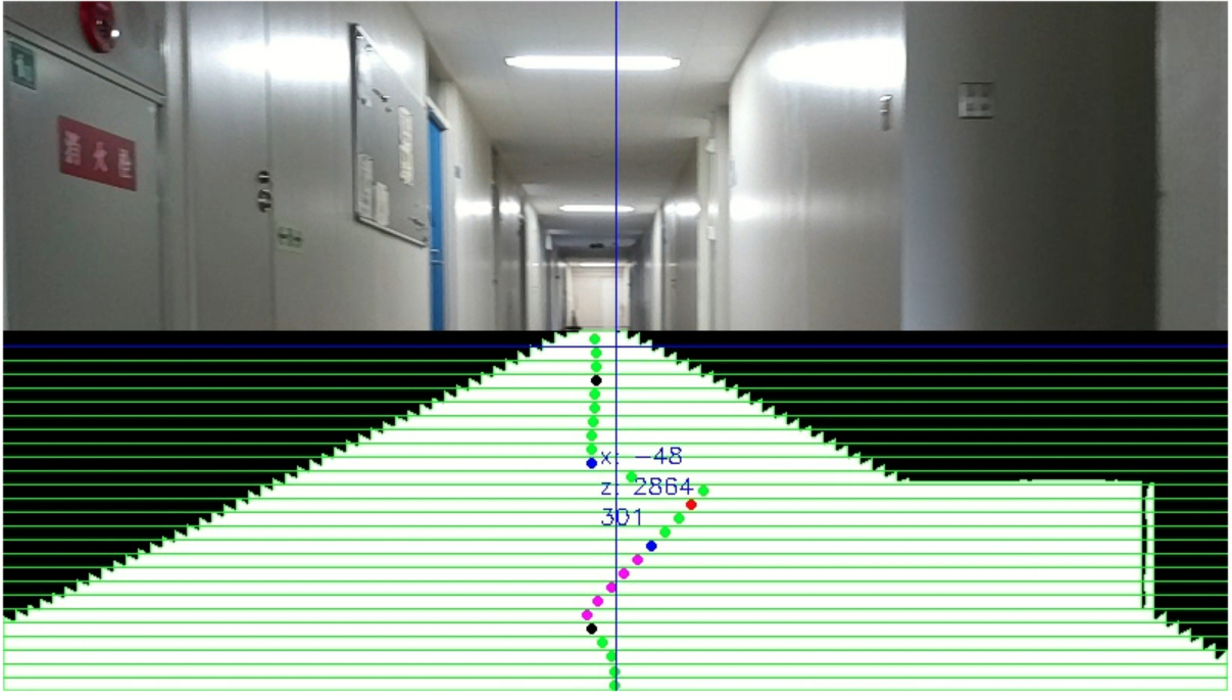
\includegraphics[scale=0.4]{./fig/case1-2.png}
	\caption{重心点の挙動の特徴の例}
	\label{fig:example}
	\end{center}
\end{figure}
%%%%%%%%%%%%%%%%%%%%%%%%
\section{\large 実機実験}
%%%%%%%%%%%%%%%%%%%%%%%%
実機実験は佐賀大学理工学1号館3回の通路で行った.{\bf Fig.~\ref{fig:ex_path2}}に示す実験経路をロボット車に走行させる.{Fig.~\ref{fig:ex_path2}}のStartを試験開始地点とし,直線$L_1$,$L_2$,$L_3$と2回の旋回を経て試験終了地点であるGoalへ到達する.
\begin{figure}[tb]
	\begin{center}
	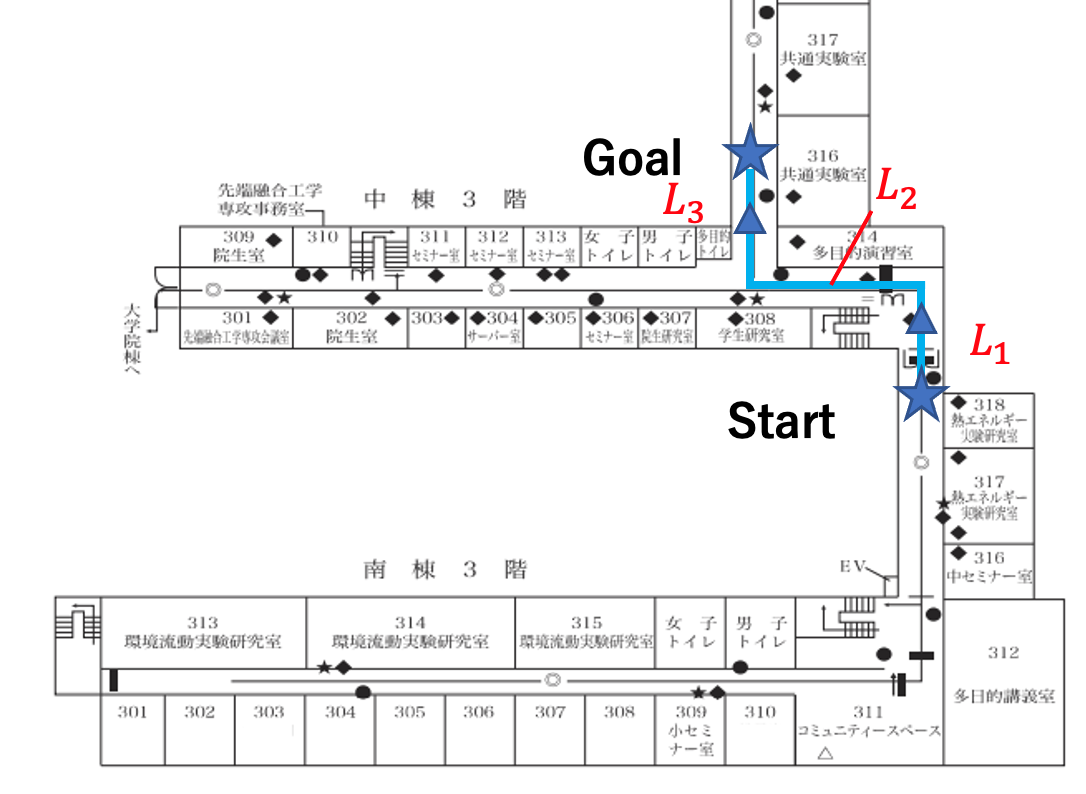
\includegraphics[scale=0.4]{./fig/ex_path2.png}
	\caption{実機実験における走行経路}
	\label{fig:ex_path2}
	\end{center}
\end{figure}
%%%%%%%%%%%%%%%%%%%%%%%%
\section{\large 考察}
%%%%%%%%%%%%%%%%%%%%%%%%

実機実験では,マーカーなどの誘導体を一切使用せずに実験経路内を自律走行し,2回の旋回動作のどちらも適切な方向に転回することができた.よって誘導体を用いず,かつカメラからの映像のみで自律走行を行うシステムは実現可能であることがわかった.本論文で提案したシステムの課題としては,旋回を行う経路が存在する場合,直進方向に経路が存在していたとしても旋回を行うこと,特殊な形状をした経路に関して,意図しない旋回が起こることが挙げられる.この問題を解決するためには,走行精度の向上と経路が直進と旋回の2つに分かれている場合,どちらを走行するか選択可能なシステムの開発が必要である.

%%%%%%%%%%%%%%%%%%%%%%%%
\section{\large 結論}
%%%%%%%%%%%%%%%%%%%%%%%%

本論文では建物内の通路を走行する移動ロボット車に関して,走行経路内に誘導体を必要としない自律走行システムの開発を行い,実機実験により,システムの有用性を検証した.今後は走行経路の床面以外の構造物の識別を行うことによって,走行精度の向上と多種多様な形状の経路での自律走行に対応させることに加え,使用者が事前に旋回指示を入力しておくことで,走行経路を指定できる方式の開発を検討している.
%%%%%%%%%%%%%%%%%%%%%%%%

\end{document}
